\section{Methodology}\label{sec:methodModel}
We have tested the model with all applications presented in Table~\ref{tab:useCases}, all of them in CUDA using the single-precision format and running a single kernel. These are: \emph{Matrix Multiplication}, \emph{Matrix Addition}, \emph{dot product}, \emph{Vector addition} and \emph{Maximum Subarray Problem} \citep{Cleber:Thesis}. For \emph{matrix multiplication}, we have used 4 different kernel strategies, and for \emph{matrix addition} we have used 2 kernel strategies. In total, we have used 9 different CUDA kernels of those matrix and vector GPU applications. The number of computation ($Comp$) and communication ($ld_0$, $st_0$, $ld_1$ and $ld_1$) steps were extracted from the application source codes, and information about cache hits in cache L1 and L2 were extracted from profiling. We also confirmed the usage of FMA and SFU using profiling. 

We have also used 6 kernels of the Rodinia applications, these kernels belong to 4 different GPU applications. These applications are: Back-propagation, Gaussian Elimination, Heartwall and Hotspot. There are applications which each execution generate one execution of the kernel and consequently a sample for our experiemnts, these are all in Table~\ref{tab:useCases} and both in the application Back propagation. Each execution of the other Rodinia applications generate multiples execution of their kernels and thus multiples samples for our experiments. During our evaluations, all applications were executed using the CUDA profile tool \textit{nvprof}. Each experiment is presented as the average of ten executions, with a confidence interval of 95\%. Only Rodinia Applications were executed on GPU Pascal. 


\textbf{\emph{Vector-Matrix Applications}}\\


For the analytical model, 69 samples of each application for problems of one dimension were taken from $2^{17}$ until $2^{28}$. From $2^{17}$ to $2^{22}$ 6 samples were taken, and from $2^{23}$ to $2^{28}$ 63 samples were collected. 32 samples of each application for problems of two dimensions were taken from $2^8$ until $2^{13}$, the input sizes or matrix sizes were vary increasing the matrix size in a step of $2^8$. Each one of the parameters of the BSP-based model were extracted from the source code of each kernel.  

For matrix multiplication versions, $Comp$ is determined by the number of multiplications and/or operations computed by a thread. In this case, each thread performs $N$ FMA single precision operations. IEEE~754-2008 floating-point standard~\citep{FMA-IEEE} states that those operations needs a single rounding step. The value of $Comp$ is the same for the all four optimizations modes, since they differ only in the memory access patterns. With those values, we can compute ---using equations \ref{ec:GM} and \ref{ec:SM}--- the values of $Comp$, $Comm_{GM}$, and $Comm_{SM}$, that are then multiplied by the number of threads $t$ in the kernel execution. 

The optimizations actually affect only the performance of the communication between threads. As explained above, $\lambda=1$ in the first execution and it is obtained by the ratio of the predicted execution time of the application with the actual measured execution time. The parameter $\lambda$ captures the effects of thread divergence, global memory access optimizations, and shared memory bank conflicts. It needs to be measures only once, for a single input size and a single board. The same lambda should work for all input sizes and boards of the same architecture. These parameters are the same for all the simulations, and are presented in Table \ref{tab:Par-NCA}.

As it was explained in Section~\ref{ssec:useCases}, each thread in both version of matrix addition request 1 element from each matrix elements and compute a single addition. The values of the parameters of the model for (MAU) and (MAC) is $Comp=1add$, $ld_1=2$, $st_1=1$, $ld_0=0$ and $st_0=0$. In the same way the parameter values of the model for (vAdd) were determined. 

The kernel of the Maximum Sub-Array Problem (MSA) is implemented using the CGM model, however it can be easily modeled with the proposed model. The scalability  of this application is also very regular. Despite the branch code divergence in the source code of this kernel, this scalability is not altered. This kernel is computed with 4096 threads, divided in 32 thread blocks with 128 threads on each. The $N$ elements are divided in intervals of $N/t$ elements, one per block and each block receive a portion of the array. The blocks use the shared memory for storing segments of its interval, which are read from the global memory using coalesced accesses.The values of the parameters of the model for (MSA) are shown in Table~\ref{tab:Par-NCA}.

\begin{table}[htpb]
\centering
\scalebox{.8}{
\begin{tabular}{| c | c | c  |  c | c | c | c | c | c | c |} 
\midrule
\multirow{2}{*}{\textbf{Par.}} & \multicolumn{4}{c|}{\textbf{Matrix 
Multiplication}}&\multicolumn{2}{c|}{\textbf{Matrix 
Addition}}&\multirow{2}{*}{\textbf{vAdd}}&\multirow{2}{*}{\textbf{dotP}}&\multirow{2}{*}{\textbf{MSA}}
\\\cline{2-7}&\textbf{MMGU}&\textbf{MMGC}&\textbf{MMSU}&\textbf{MMSC}&\textbf{MAU}&\textbf{MAC}&&\\\midrule
$\mathbf{comp}$&\multicolumn{4}{c|}{$N\cdot$ FMA}&\multicolumn{3}{c|}{$1\cdot 24$}&$1\cdot 96$&$(N/t)\cdot{}100 $\\\midrule
$\mathbf{ld_1}$&\multicolumn{4}{c|}{$2\cdot N$}&\multicolumn{3}{c|}{2}&2&$N/t$\\\midrule
$\mathbf{st_1}$&\multicolumn{4}{c|}{1}&\multicolumn{3}{c|}{2}&$1/GS$&$5$\\\midrule
$\mathbf{ld_0}$&\multicolumn{2}{c|}{0}&\multicolumn{2}{c|}{$2\cdot N$}&\multicolumn{3}{c|}{0}&$1 + 2\cdot{}log(BS)$&$2\cdot{}(N/t)$\\\midrule
$\mathbf{st_0}$&\multicolumn{2}{c|}{0}&\multicolumn{2}{c|}{1}&\multicolumn{3}{c|}{0}&$1 + 2\cdot{}log(BS)$&$N/BS^2$\\
\midrule
\end{tabular}}
\caption{Values of the model parameters over 9 different vector/matrix applications}
\label{tab:Par-NCA} % is used to refer this table in the text
\end{table}

Different micro-benchmarks were used to measure the number of cycles per computation operation in GPUs~\citep{Bench:GPU}, with FMAs, additions, multiplications, divisions,  taking approximately 8, 16, 32 and up to 96 cycles of clock. For all simulations, we considered $5$ cycles for latency in the communication for shared memory and $500$ cycles for global memory \citep{CUDAGuide}. Finally, when the models were complete, we executed a single average instance of each application on each GPU to determine the $\lambda$ values. As explained above, $\lambda=1$ in the first execution and it is obtained by the ratio of the predicted execution time of the application with the actual measured execution time. Finally, for the parameter $\lambda$, which captures the effects of thread divergence, global memory access optimizations, and shared memory bank conflicts, we used the values described in Table~\ref{tab:Lambda-NCA}. 

\begin{table}[htpb]
\centering
\scalebox{0.8}{
\begin{tabular}{| c | c | c  |  c | c | c | c | c | c | c |} 
\hline \hline
\multirow{2}{*}{\textbf{\backslashbox{GPUs}{Kernels}}}& \multicolumn{4}{c|}{\textbf{Matrix Multiplication}}& \multicolumn{2}{c|}{\textbf{Matrix Addition}}&\multirow{2}{*}{\textbf{vAdd}}&\multirow{2}{*}{\textbf{dProd}}&\multirow{2}{*}{\textbf{MSA}} \\\cline{2-7}
&\textbf{MMGU}&\textbf{MMGC}&\textbf{MMSU}&\textbf{MMSC}&\textbf{MAU}&\textbf{MAC}\\\hline
GTX-680 &\cellcolor{green!50} 4.50 &\cellcolor{green!50} 19.00 &\cellcolor{green!50} 20.00 &\cellcolor{green!50} 68.00 &\cellcolor{green!50} 1.50 &\cellcolor{green!50} 9.25 &\cellcolor{green!50} 14.00 &\cellcolor{green!50} 11.00 &\cellcolor{green!50} 0.68 \\ 
  Tesla-K40 &\cellcolor{green!50} 4.30 &\cellcolor{green!50} 20.00 &\cellcolor{green!50} 19.00 &\cellcolor{green!50} 65.00 &\cellcolor{green!50} 2.50 &\cellcolor{green!50} 9.50 &\cellcolor{green!50} 5.50 &\cellcolor{green!50} 10.00 &\cellcolor{green!50} 0.48 \\ 
  Tesla-K20 &\cellcolor{green!50} 4.50 &\cellcolor{green!50} 21.00 &\cellcolor{green!50} 18.00 &\cellcolor{green!50} 52.00 &\cellcolor{green!50} 2.50 &\cellcolor{green!50} 9.00 &\cellcolor{green!50} 6.00 &\cellcolor{green!50} 10.00 &\cellcolor{green!50} 0.55 \\ 
  Titan &\cellcolor{green!50} 4.25 &\cellcolor{green!50} 21.00 &\cellcolor{green!50} 17.00 &\cellcolor{green!50} 50.00 &\cellcolor{green!50} 2.50 &\cellcolor{green!50} 10.00 &\cellcolor{green!50} 5.50 &\cellcolor{green!50} 12.00 &\cellcolor{green!50} 0.48 \\ 
Quadro &\cellcolor{green!50} 4.75 &\cellcolor{green!50} 20.00 &\cellcolor{green!50} 20.00 &\cellcolor{green!50} 64.00 &\cellcolor{green!50} 1.50 &\cellcolor{green!50} 8.25 &\cellcolor{green!50} 11.00 &\cellcolor{green!50} 9.50 &\cellcolor{green!50} 0.55 \\
  TitanX & 9.50 & 36.00 & 36.00 & 110.00 & 3.00 & 9.50 & 7.00 & 9.75 & 0.95 \\ 
  GTX-970 & 13.00 & 44.00 & 46.00 & 120.00 & 3.75 & 9.50 & 8.00 & 10.50 & 1.95 \\ 
  GTX-980 & 13.00 & 44.00 & 46.00 & 120.00 & 3.25 & 9.50 & 7.00 & 9.50 & 1.50 \\\hline
\end{tabular}}
\caption{Values of the parameter $\lambda$ for each vector/matrix CUDA kernel in the GPUs used}
\label{tab:Lambda-NCA} % is used to refer this table in the text
\end{table}

The Values of $\lambda$ for each application and each GPU is shown in Table~\ref{tab:Lambda-NCA} and graphically in Figure~\ref{fig:LambdaNCA}. Green Cells in Table~\ref{tab:Lambda-NCA} groups the values of $\lambda$ by GPU architectures, those without color belong to Maxwell architecture and those of green are Kepler architectures. The same lambda should work for all input sizes and boards of the same architecture. The box plots of Figure~\ref{fig:LambdaNCA} show the median for each application in all the GPUs and the upper and lower first quartiles, with whiskers representing the 95\% confidence interval. Outliers are marked as individual points.

\begin{figure}[htpb]
\centering
 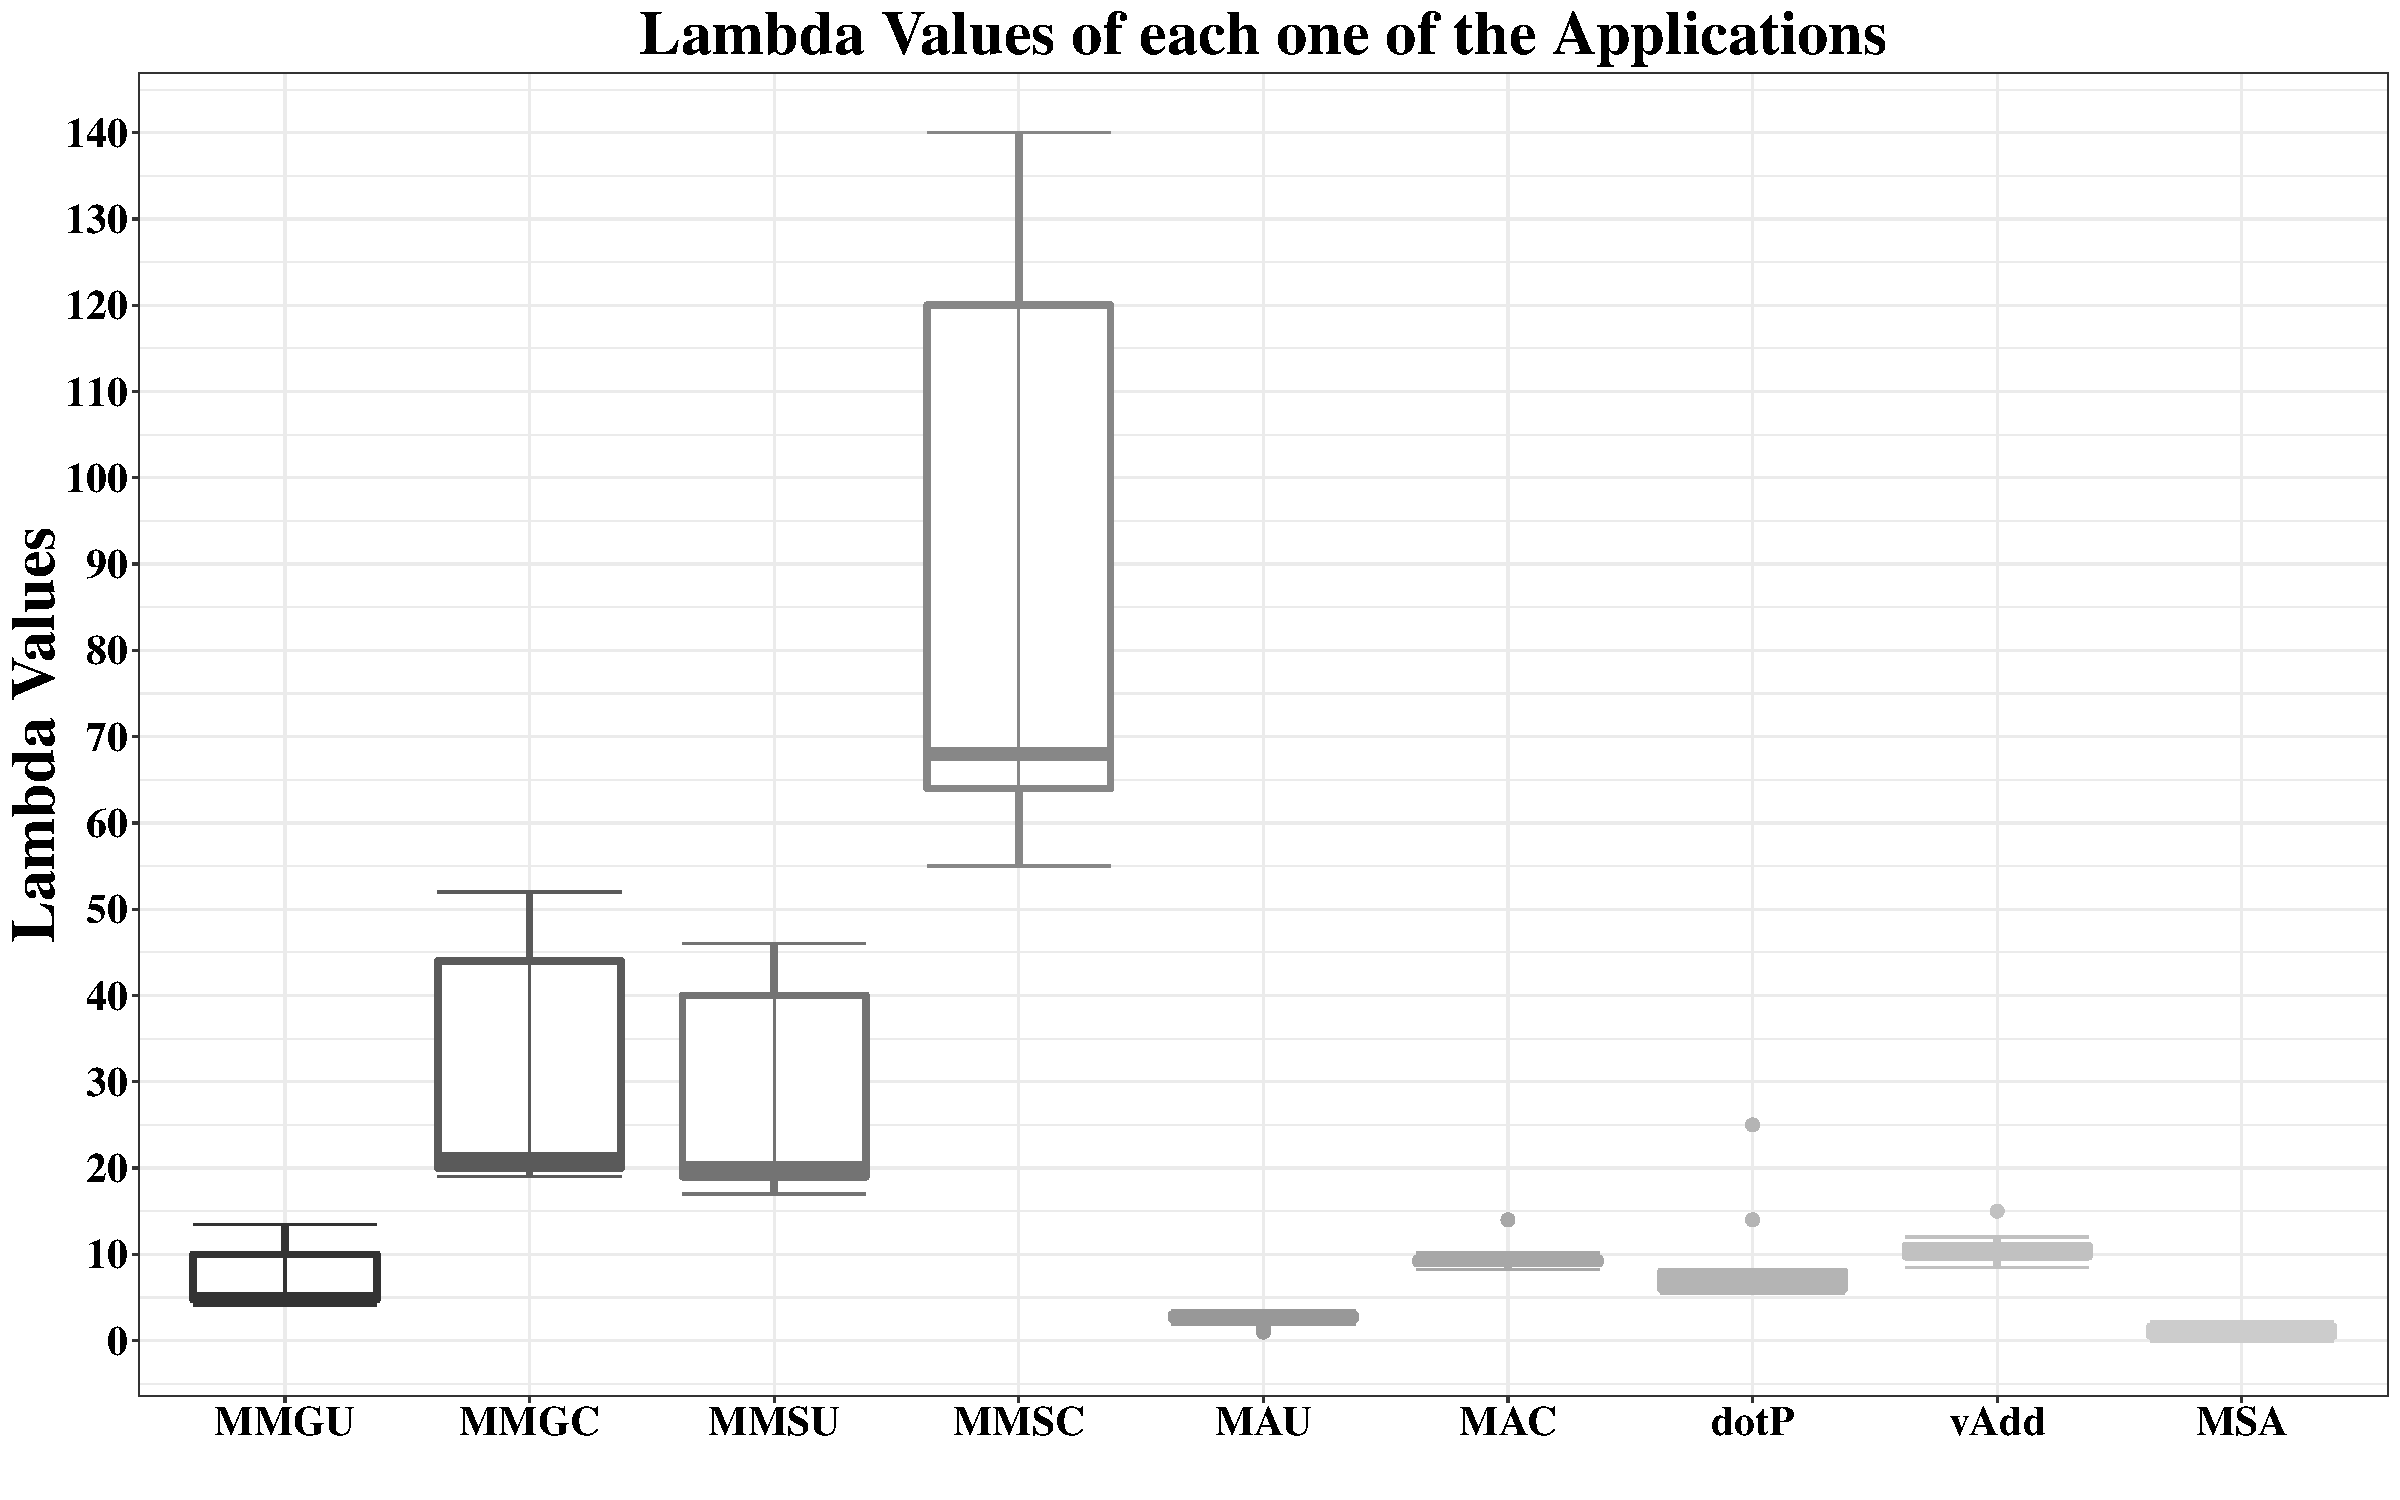
\includegraphics[scale=.3]{./images/LambdaAnalyticalModel-NCA.pdf}
\caption{Boxplot of $\lambda$ values, see table~\ref{tab:Lambda-NCA}}
\label{fig:LambdaNCA}
\end{figure}

\textbf{\emph{Rodinia Benchmark Applications}}\\
Our analytical model was tested with 4 Rodinia algorithms, Back-propagation, Gaussian Elimination, Heartwall and Hotspot. The number of samples of each application is shown in Table~\ref{tab:Rodinia}. Similarly to the vector/matrix applications mentioned before, the variables of computation ($Comp$) and communication ($ld_0$, $st_0$, $ld_1$ and $ld_1$) were extracted from the application source codes. For kernel (HWL), it was not possible to know the values of the parameters of the analytical model, due to the large number of code lines. For this reason the values of the parameters for the analytical model were extracted from profile information. These values are presented in Table~\ref{tab:Par-Rodinia}.  Kernel (HWL) uses constant memory to store large numbers of parameters which cannot be readily fit into shared memory, resulting in a high number of instructions over the global memory. Finally, when values of the parameters of the models were completed, we executed a single instance of each application on each GPU to determine the $\lambda$ values. As explained above, $\lambda=1$ in the first execution and it is obtained by the ratio of the predicted execution time of the application with the actual measured execution time. 

\begin{table}[htpb]
\centering

\begin{tabular}{| c | c | c  |  c | c | c | c |} 
\midrule
\multirow{2}{*}{\textbf{Par.}} & \multicolumn{2}{c|}{\textbf{Back propagation}}&\multicolumn{2}{c|}{\textbf{Gaussian}}&\multirow{2}{*}{\textbf{HWL}}&\multirow{2}{*}{\textbf{HOT}}
\\\cline{2-5}& \textbf{BCK-1} & \textbf{BCK-2} & \textbf{GAU-1} & \textbf{GAU-2} & &   \\\midrule
$\mathbf{comp}$&404&116&36&96&7600000&500 \\\midrule
$\mathbf{ld_1}$&2&4&1&3&7000&2\\\midrule
$\mathbf{st_1}$&1/GS&1&1&1&2000&1\\\midrule
$\mathbf{ld_0}$&BS&0&0&0&2800&2\\\midrule
$\mathbf{st_0}$&BS&0&0&0&1&1\\
\midrule
\end{tabular}
\caption{Values of the model parameters over 6 CUDA kernels of Rodinia Benchmark Suite}
\label{tab:Par-Rodinia} % is used to refer this table in the text
\end{table}

Finally, for the parameter $\lambda$ of the Rodinia CUDA kernel, which captures the deep thread and memory hierarchy, we used the values described in Table~\ref{tab:lambdaRodinia}. These values are also shown graphically in Figure~\ref{fig:LambdaRodinia}. This table present three different groups, they are green, blue and without color, which group GPU architecture which are Kepler, Maxwell and Pascal architectures, respectively. It is easy also to notice that values of the $\lambda$ parameter have less variance when belong to the same architecture.



\begin{table}[htpb]
\centering
\begin{tabular}{|r|c|c|c|c|c|c|}
  \hline
 \textbf{\backslashbox{GPUs}{Kernels}}& BCK-1 & BCK-2 & GAU-1 & GAU-2 & HWL & HOT  \\ 
  \hline
    GTX-680 &\cellcolor{green!50} 6.2 &\cellcolor{green!50} 7.50 &\cellcolor{green!50} 0.26 &\cellcolor{green!50} 0.65 &\cellcolor{green!50} 2.15 &\cellcolor{green!50} 8.00 \\ 
  Tesla-K40 &\cellcolor{green!50} 6.30 &\cellcolor{green!50} 8.50 &\cellcolor{green!50} 0.35 &\cellcolor{green!50} 1.25 &\cellcolor{green!50} 2.25 &\cellcolor{green!50} 14.00 \\ 
  Tesla-K20 &\cellcolor{green!50} 6.4 &\cellcolor{green!50} 8.50 &\cellcolor{green!50} 0.35 &\cellcolor{green!50} 1.25 &\cellcolor{green!50} 2.50 &\cellcolor{green!50} 14.50 \\ 
  Titan &\cellcolor{green!50} 6.2 &\cellcolor{green!50} 8.50 &\cellcolor{green!50} 0.35 &\cellcolor{green!50} 1.25 &\cellcolor{green!50} 2.25 &\cellcolor{green!50} 14.00 \\ 
  Quadro &\cellcolor{green!50} 5.60 &\cellcolor{green!50} 7.00 &\cellcolor{green!50} 0.25 &\cellcolor{green!50} 0.70 &\cellcolor{green!50} 1.65 &\cellcolor{green!50} 8.00 \\ 
  TitanX &\cellcolor{blue!25} 4.20 &\cellcolor{blue!25} 5.50 &\cellcolor{blue!25} 0.40 &\cellcolor{blue!25} 2.00 &\cellcolor{blue!25} 3.25 &\cellcolor{blue!25} 7.00 \\ 
  GTX-970 &\cellcolor{blue!25} 5.60 &\cellcolor{blue!25} 6.50 &\cellcolor{blue!25} 0.70 &\cellcolor{blue!25} 3.50 &\cellcolor{blue!25} 5.00 &\cellcolor{blue!25} 8.00 \\ 
  GTX-980 &\cellcolor{blue!25} 4.5 &\cellcolor{blue!25} 5.75 &\cellcolor{blue!25} 0.45 &\cellcolor{blue!25} 2.50 &\cellcolor{blue!25} 3.75 &\cellcolor{blue!25} 7.00 \\
  Tesla-P100 & 8.40 & 10.50 & 0.30 & 2.00 & 5.50 & 25.00 \\ 
   \hline
\end{tabular}
\caption{Values of the parameter $\lambda$ for each Kernels of the Rodinia Benchmark in the GPUs used}
\label{tab:lambdaRodinia}
\end{table}

In all experiments, we modeled only communication over global memory and shared memory. We did not include the values of the cache L2 for these experiments because they did not impact the variance of the execution times. And $L1$ caching in Kepler, Maxwell and Pascal architectures is reserved for register spills in local memory. For this reason $L1$ and $L2$ are always 0 for all the experiments. Cache effects are hard to predict and its impact is higher for specific applications and problem sizes. For example, small vector/matrix problems can profit more from L1 cache memory. This happens in applications which do not use shared memory and their accesses to the global memory are uncoalesced, since they can exploit the cache line size and load multiple elements in the same transaction~\citep{Wu:2013:Coalesced}.

\begin{figure}[htpb]
\centering
 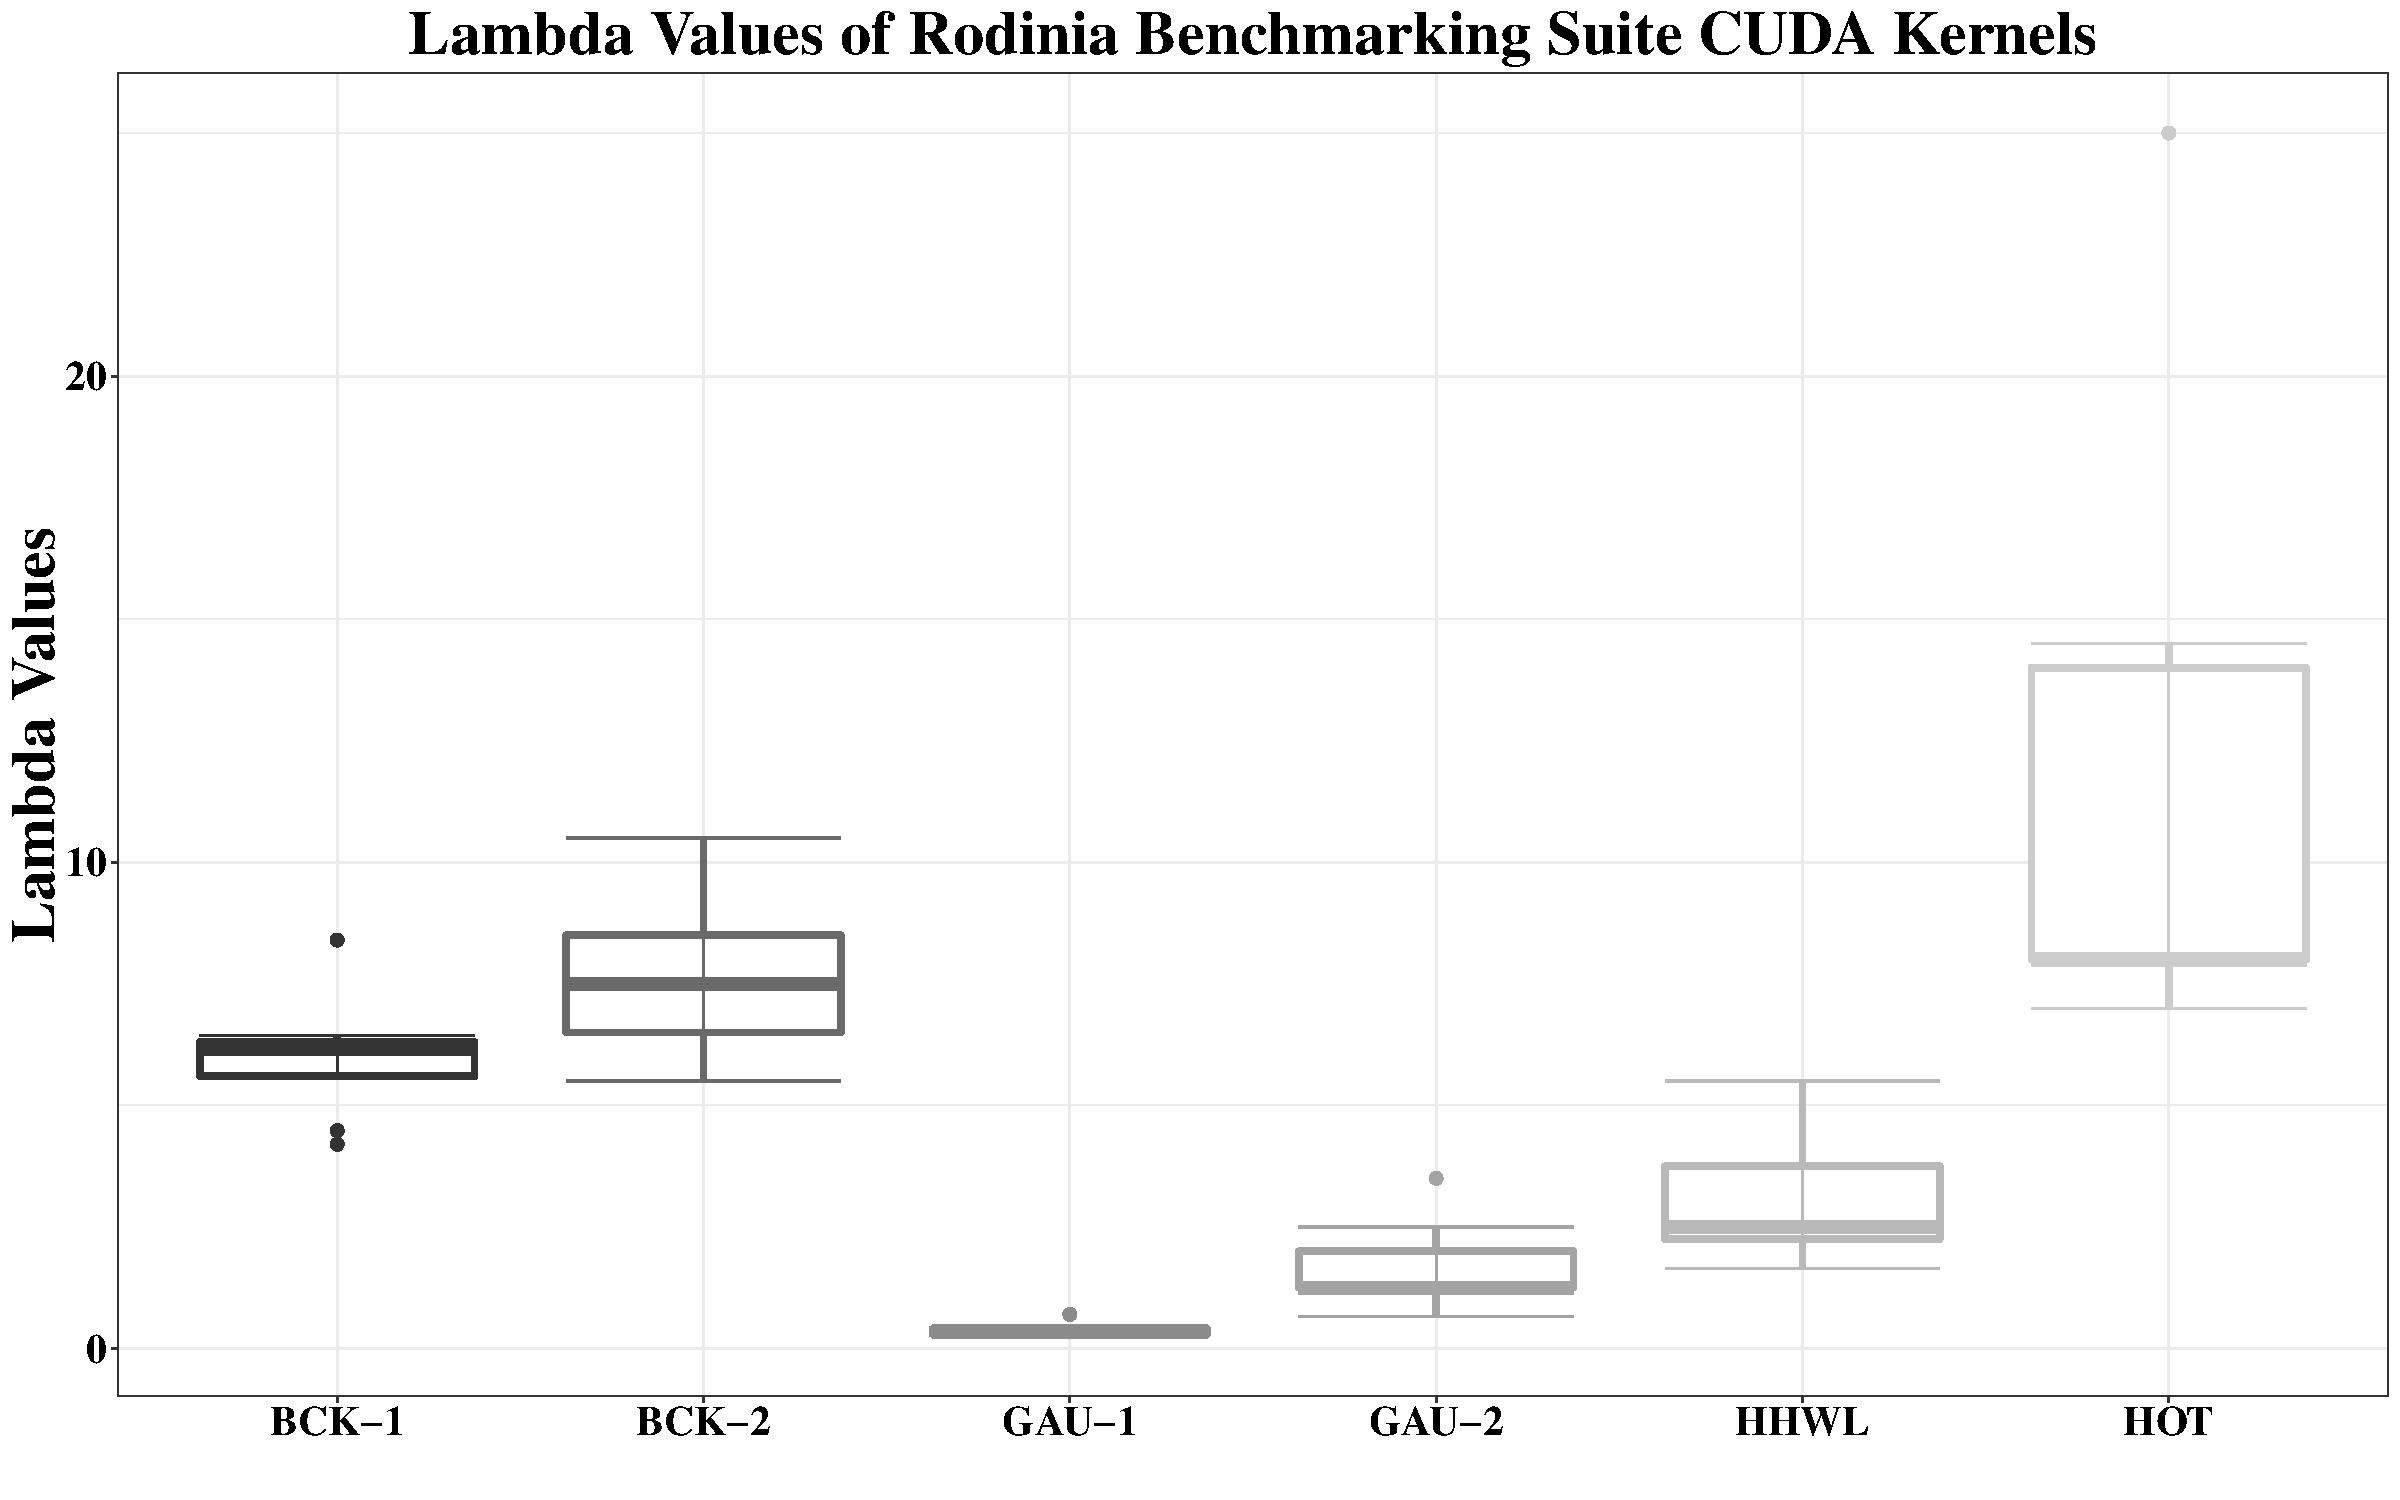
\includegraphics[scale=.3]{images/LambdaAnalyticalModel-Rodinia.pdf}
\caption{Boxplot of $\lambda$ values of Rodinia CUDA Kernels, see table~\ref{tab:lambdaRodinia}}
\label{fig:LambdaRodinia}
\end{figure}
% Note that higher optimizations levels results in larger $\lambda$ values and, consequently, the $\lambda$ can bwe considered an estimator of the application optimization level. 

We have used our analytical model in some Rodinia Applications, for them which the analytical model was adequate. The proposed BSP-based analytical model is useful for those applications which its scalability is regular with the input parameters. When kernels iterate in an application and the number of threads and divergence change on each iteration, it makes difficult to predict the running time of different CUDA kernels. Machine learning can be a solution for this type of kernels, in Chapter~\ref{Chap:ML} we describe a implementation of machine learning techniques for these kernels in two different approaches. Another option would be to use other analytical models which are explained in Section~\ref{sec:relatedModel} of this chapter.


